% OLD
%\documentclass[11pt,compress,t,notes=noshow, aspectratio=169, xcolor=table]{beamer}
% NEW
\documentclass[10pt,compress,t,notes=noshow, xcolor=table]{beamer}

% Defines macros and environments
% includepdf slides, pagecommad will set counter for framenumber

\input{../../style/preamble}
\input{../../latex-math/basic-math}
\input{../../latex-math/basic-ml}

\setbeamersize{text margin left=0.3cm,text margin right=0.3cm}


\usepackage{pdfpages}
\includepdfset{trim=0mm 0mm 0mm 0mm, pagecommand={\global\setcounter{framenumber}{\value{page}}}}
% trim=0mm 6mm 0mm 0mm, offset=0 15,
% add footer:
\usepackage{framed, color}
\usepackage{xcolor}


\title{Applied Machine Learning}
% \author{LMU}
%\institute{\href{https://compstat-lmu.github.io/lecture_iml/}{compstat-lmu.github.io/lecture\_iml}}
\date{}

\begin{document}

\titlemeta{
PLACEHOLDER
}{
Feature Engineering
}{
figure/empty
}{
\item Categorical Encoding: \newline One-Hot and Target/Impact Encoding
\item Feature Transformations: \newline Normalization and Box-Cox Transformation
\item Intro to mlr3pipelines
}



\section{Introduction to Feature Engineering}
\includepdf[pages={3}]{pdf_chapters/slides_intro_fe.pdf}
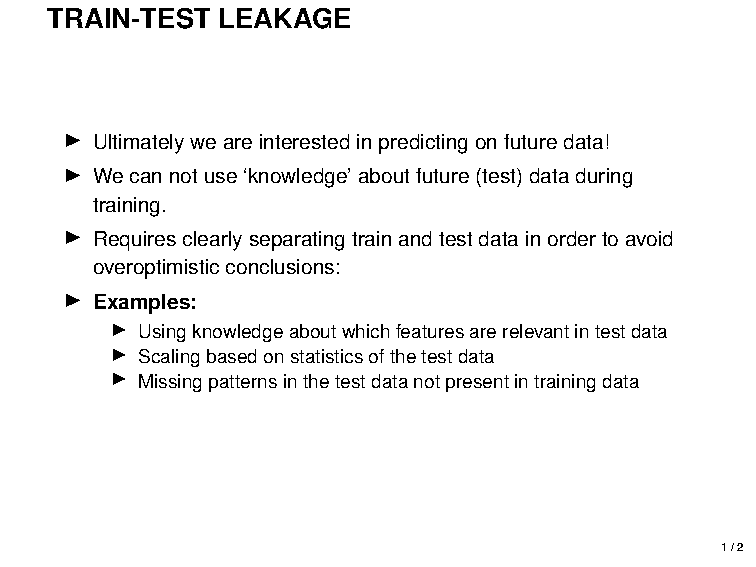
\includepdf[pages={1-last}]{pdf_chapters/slides_leakage.pdf}
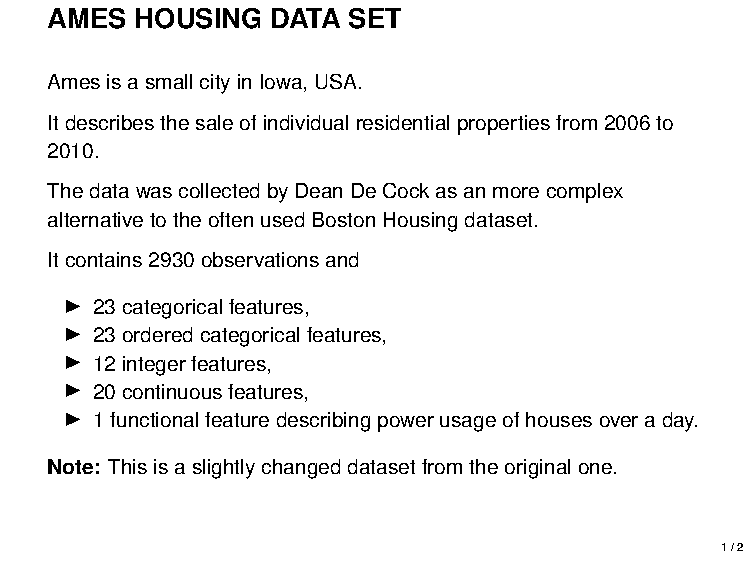
\includepdf[pages={1-last}]{pdf_chapters/slides_ames_extended.pdf}
\section{Handling of Categorical Features}
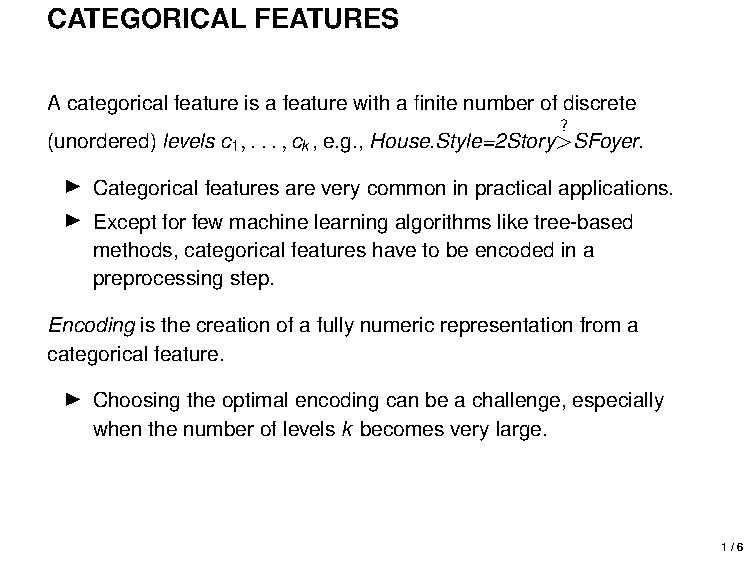
\includepdf[pages={1-4, last}]{pdf_chapters/slides_categ_encode_dummy.pdf}
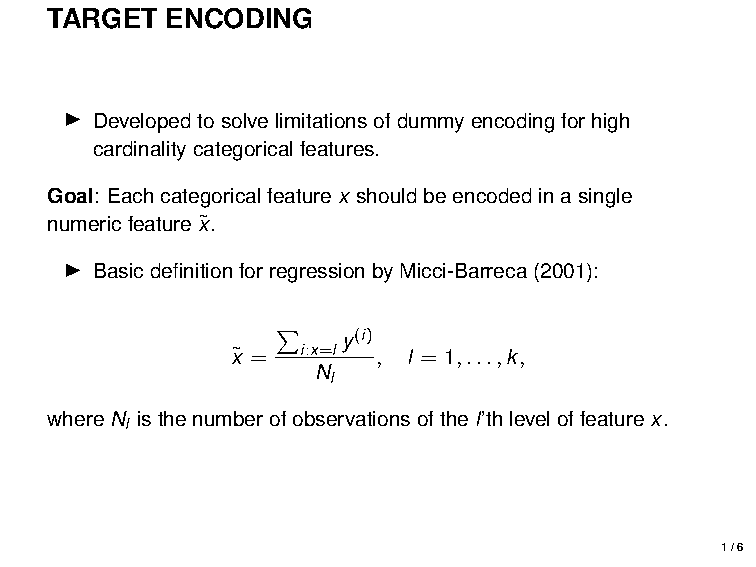
\includepdf[pages={1-last}]{pdf_chapters/slides_categ_encode_impact.pdf}
\section{Feature Transformation}
%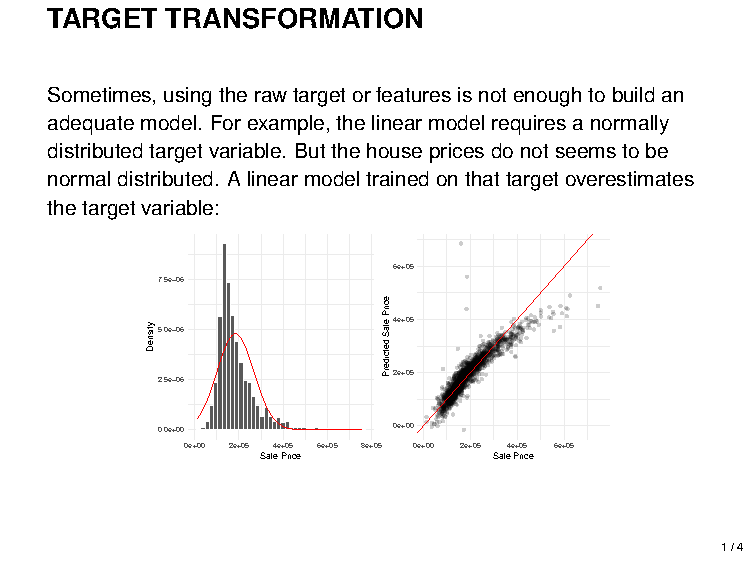
\includepdf[pages={1-last}]{pdf_chapters/slides_01_ftt_target.pdf}
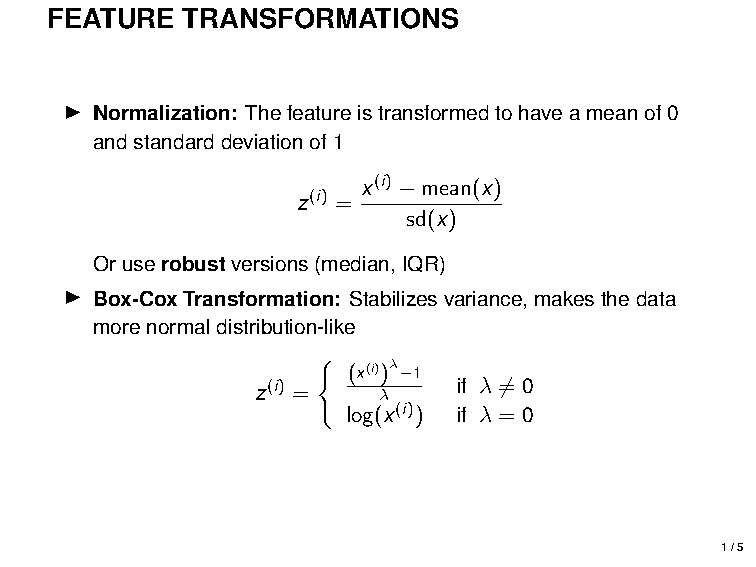
\includepdf[pages={1-last}]{pdf_chapters/slides_02_ftt_feature_trafos.pdf}
% \section{Imputation}
% \includepdf[pages={3-last}]{pdf_chapters/slides_01_imputation_intro.pdf}
% 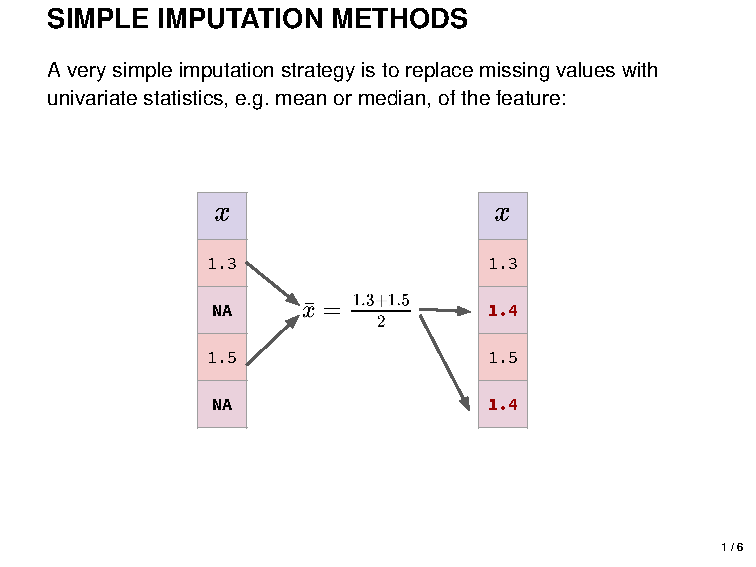
\includepdf[pages={1-5}]{pdf_chapters/slides_02_imputation_simple.pdf}
% 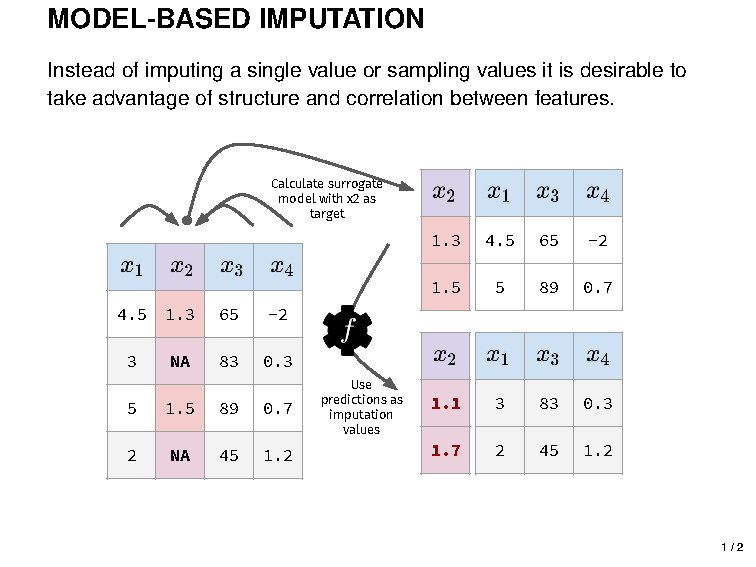
\includepdf[pages={1-last}]{pdf_chapters/slides_03_imputation_models.pdf}
\section{mlr3pipelines: Introduction}

\includepdf[pages={4-8, 10-13, 15-16, 21, 25}]{../mlr3slides/mlr3pipelines.pdf}
%\section{Overview of PipeOps}
%
\includepdf[pages={59-60, 17-18}]{../mlr3slides/mlr3pipelines.pdf}
%\section{mlr3pipelines: Graph Operations} % gunion and greplicate
%
\includepdf[pages={21-23, 25}]{../mlr3slides/mlr3pipelines.pdf}
\section{mlr3pipelines: Linear Pipelines}

\includepdf[pages={27-33, 36}]{../mlr3slides/mlr3pipelines.pdf}
\endlecture
\end{document}
